\documentclass[10pt,xcolor=table]{beamer}
%\usepackage{natbib}
%\mode<presentation> {
%    \usetheme{sptl}
%    \usecolortheme{default}
%    \usefonttheme{serif}
%    \setbeamertemplate{navigation symbols}{}
%    \setbeamertemplate{caption}[numbered]
%}
% Use the preamble setting
% Beamer theme
%\usetheme{sptl}
\mode<presentation>
{
	\usetheme{sptl}
	%\usecolortheme{default}
	\usefonttheme{serif}
	%\setbeamertemplate{navigation symbols}{}
	%\setbeamertemplate{caption}[numbered]
} 

% Settings to have progress bar at the top
\useoutertheme[subsection=false]{miniframes}
\useinnertheme{circles}
%% \usefonttheme{structurebold}
\usecolortheme{beaver}

% Some change in font colour
\setbeamercolor{normal text}{fg=black, bg=white}
\setbeamercolor{altered text}{fg=black, bg=white}
\setbeamercolor{example text}{fg=black, bg=white}

% Change in the title color
\definecolor{bured}{rgb}{0.8, 0.0, 0.0}
\setbeamercolor{frametitle}{fg=bured, bg=bured!10}

% Add graphics path
\usepackage{graphicx}
\graphicspath{{images/}}

\usepackage{booktabs}
\usepackage[scale=2]{ccicons}

%\usepackage{enumitem}
\usepackage{xcolor}
\setbeamercolor{itemize item}{fg=bured}
\setbeamercolor{local structure}{fg=bured}

\usepackage{pgfplots}
\usepgfplotslibrary{dateplot}
\pgfplotsset{compat=1.18}
% Define graphics for logo
\titlegraphic{%
    \begin{figure}[b]
        
\includegraphics[height=.125\textheight]{BostonUni.png} \hfill
        
\includegraphics[height=.125\textheight]{images/sptl_v2.png}
    \end{figure}
  
}

% Set the log to appear on all screens
\usepackage{transparent}
\logo{{\transparent{0.2}
\includegraphics[height=.125\textheight]{sptl_v2.png}}}

% Method to add an item that will appear in every slide
% \addtobeamertemplate{footline}{%
%   \setlength\unitlength{1ex}%
%   \begin{picture}(1,1) 
%     % \put{} defines the position of the frame
%     \put(1,6){\makebox(0,0)[bl]{
%     
\includegraphics[height=.125\textheight]{images/sptl_v2.png}
%     }}%
%   \end{picture}%
% }{}

% Setting title page to be centered, and add logos at the bottom
\makeatletter
\setbeamertemplate{title page}{
  \begin{minipage}[b][\paperheight]{\textwidth}
    % Centering titles    
    \centering  % <-- Center here
    \vfill%
    \ifx\inserttitle\@empty\else\usebeamertemplate*{title}\fi
    \ifx\insertsubtitle\@empty\else\usebeamertemplate*{subtitle}\fi
    \usebeamertemplate*{title separator}
    \ifx\beamer@shortauthor\@empty\else\usebeamertemplate*{author}\fi
    \ifx\insertdate\@empty\else\usebeamertemplate*{date}\fi
    \ifx\insertinstitute\@empty\else\usebeamertemplate*{institute}\fi
    \vfill
    % Inserting logo
    \ifx\inserttitlegraphic\@empty\else\inserttitlegraphic\fi    
    \vspace*{10mm}
  \end{minipage}
  
}
\setbeamertemplate{title}{
%  \raggedright%  % <-- Comment here
  \linespread{1.0}%
  \inserttitle%
  \par%
  \vspace*{0.5em}
}
\setbeamertemplate{subtitle}{
%  \raggedright%  % <-- Comment here
  \insertsubtitle%
  \par%
  \vspace*{0.5em}
}
\makeatother

% Manage frame numbering in beamer's appendixes
\usepackage{appendixnumberbeamer}

% references
% \usepackage{cleveref}

% URL
\usepackage{hyperref}
\hypersetup{
    colorlinks=true,
    linkcolor=black,
    citecolor=blue,
    filecolor=magenta,      
    urlcolor=magenta,
    pdfpagemode=FullScreen,
    }

% Citation
%style options = "numeric", "alphabetic", "authoryear", "authortitle", "verbose", "reading"
% Check this link for more options: "https://www.overleaf.com/learn/latex/Biblatex_citation_styles"
\usepackage[backend=bibtex,style=alphabetic]{biblatex}

% Change caption font size
\usepackage[font=scriptsize, labelfont=bf]{caption}
\usepackage{subcaption}

% Box around text
\usepackage{tcolorbox}

% For large table in the timeline
\usepackage{chngpage}


% Title and logo
\title[A shorter title]{Some Title for Presentation on some Random Research Topic}
\subtitle[test]{Some other details related to subtitle}
\date{\today}
\author[alphazeta@bu.edu]{Alpha B. Zeta}
\institute[SPTL, BU]{Center for Space Physics, Boston University}

% Add bibliography file. You can change bibliography style in preamble.tex file.
\bibliography{bibliographies/Papers}

\begin{document}

% Make the title
{
% Uncomment the following to dismiss the transparent background crest
\setbeamertemplate{background}{\tikz[remember picture,overlay]\node[opacity=0.04] at (current page.center) {
\includegraphics[height=0.8\paperheight,keepaspectratio]{BostonUni_Crest.eps}};}
\maketitle
}

%\begin{frame}
%	\titlepage
%	\begin{center}
%	\textbf{Arcetri Meeting}
%	\end{center}
%
%\end{frame}

% Setting all titles to be centered
%\setbeamertemplate{frametitle}[default][center]

% Table of content
\begin{frame}[plain]{Table of Contents}
  \setbeamertemplate{section in toc}[sections numbered]
  %\tableofcontents[hideallsubsections]
  \tableofcontents[currentsubsection,sectionstyle=show,subsectionstyle=show/shaded]
\end{frame}

% Section 1
\section[Intro]{Introduction}
    \begin{frame}{A simple sample for a slide}
        \begin{itemize}
            \item Something important goes here.
            \item This is the other bullet point.
            \item can change the bullet style
        \end{itemize}
    \end{frame}
    
    \begin{frame}{List of objects using enumerate}
        How to itemize a list with different options:
        \begin{enumerate} %Options: [I], [(a)], 
            \item You can use [I] for numbering in upper case Roman numerals
            \item Use this [(a)] for numbering by letters
        \end{enumerate}
    
        \begin{itemize}
            \item This is the default bullet option
            \item[!] A point to exclaim something!
            \item[$\blacksquare$] Make the point fair and square.
            \item[NOTE] This entry has no bullet
            \item[] A blank label?
        \end{itemize}
    \end{frame}


\begin{frame}
    How to show a specific text or image on only one slide?
    % On all slides
	\begin{center}
		\includegraphics[width=1.5in]{images/lexi_01.jpg}\hspace{0.25in}
	\end{center}
	% Only on the first slide
	\onslide<1>{
	    \begin{align*}
	        Author~et~al.~~(\textit{Journal}, 2022)\\
	        \rm{This~is~only~on~slide~1}
	    \end{align*}
	    }
	% On slide 2 and 3 to the last slide
	\onslide<1-2>{
		\vspace{-0.2in}
		\begin{itemize}
			\item This item is only on slide 1 and 2.
		\end{itemize}
	}
	\onslide<3->{On slide 3 and above}
\end{frame}

\begin{frame}
  \frametitle{Unusual layout frame}
  \begin{columns}
    \begin{column}{.44\textwidth}
      \begin{figure}[t]
        \includegraphics[width=0.8\textwidth]{lexi_01.jpg}
        \caption{A picture of a LEXI\footnotemark[1].}
      \end{figure}
    \end{column}
    \begin{column}{.60\textwidth}
      Observations:
        \begin{itemize}
        \item A picture of instrument.
        \item It looks good.
        \end{itemize}
        \end{column}
    \end{columns}

  You can also split things into two columns and arrange them as so.
  
  \vspace{0.8cm}
\end{frame}

% Section 2
\section{Methodology}
\begin{frame}
  \frametitle{How to perform research}
  \begin{figure}
    \includegraphics[width=0.5\textwidth]{lexi_01.jpg}
    \caption{Hedgehog posing in a tiny kayak.}
  \end{figure}
  \vspace{-0.4cm}
  \begin{itemize}
  \item This is a picture of a happy hedgehog.
  \item You can even cite where this hedgehog is from.
  \end{itemize}
  \vspace{0.15cm}
\end{frame}

\begin{frame}
  \frametitle{Concurrent vs Information-passing}
  \begin{columns}
    \begin{column}{0.5\textwidth}
      \begin{figure}
        \includegraphics[width=0.45\textwidth]{lexi_01.jpg}
        \caption{Gecko strumming a leaf\footnotemark[2].}
      \end{figure}
      \begin{itemize}
      \item He pulled out his guitar:
      \item `Anyway, here's Wonderwall.'
      \end{itemize}
    \end{column}
    \begin{column}{0.5\textwidth}
      \begin{figure}
        \includegraphics[width=0.45\textwidth]{lexi_01.jpg}
        \caption{Bald eagle over ice\footnotemark[3].}
      \end{figure}
      \begin{itemize}
      \item `\textit{When will my reflection shows...}'
      \item `\textit{...who I am, inside}.'
      \end{itemize}      
    \end{column}    
  \end{columns}
  \vspace{0.25cm}
  % Again, fix for the citation at the bottom
\end{frame}


% Results
\section{Results}
\begin{frame}
  \frametitle{Computer models and calibration}
  \begin{itemize}
  \item Some results here...
  \item Some results there...
  \item And happy dancing mantis!
  \end{itemize}  
  %\begin{figure}
  %  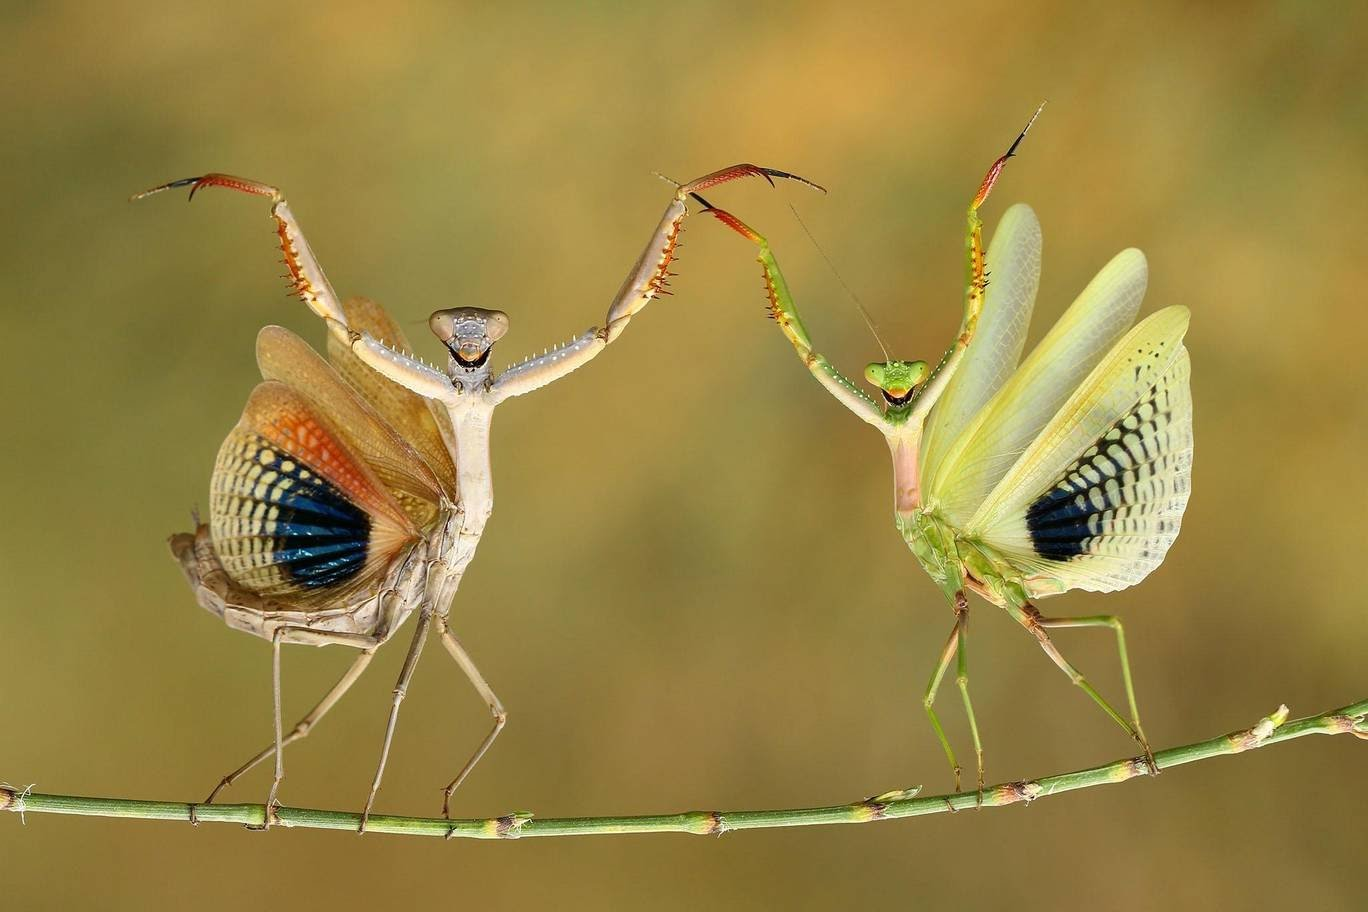
\includegraphics[width=0.65\textwidth]{mantis}
  %  \caption{Two mantis on a wig.}
  %\end{figure}
\end{frame}

% Some more results
\section{Some more results}
\begin{frame}
  \frametitle{More Results}
  \begin{itemize}
  \item This is an interesting result
  \item We need to talk more about it
  \end{itemize}
\end{frame}

% Some more results
\section{Some serious results}
\begin{frame}
  \frametitle{More Results}
  \begin{itemize}
  \item This is an interesting result
  \item We need to talk more about it
  \end{itemize}
\end{frame}

\begin{frame}
  \frametitle{More Results}
  \begin{itemize}
  \item This is an interesting result
  \item We need to talk more about it
  \end{itemize}
\end{frame}
\begin{frame}
  \frametitle{More Results}
  \begin{itemize}
  \item This is an interesting result
  \item We need to talk more about it
  \end{itemize}
\end{frame}
\begin{frame}
  \frametitle{More Results}
  \begin{itemize}
  \item This is an interesting result
  \item We need to talk more about it
  \end{itemize}
\end{frame}
% Some more results
\section{Some more serious results}
\begin{frame}
  \frametitle{More Results}
  \begin{itemize}
  \item This is an interesting result
  \item We need to talk more about it
  \end{itemize}
\end{frame}


% Conclusion and Further work
\section{Conclusion and Further work}
\begin{frame}
  \frametitle{Remarks}
  \begin{itemize}
  \item The first goal is working hard.
  \item The second goal is working a bit harder.
  \item The most important goal is, however, having fun.
  \item And you also get called a doctor by the end of it.
  \end{itemize}
\end{frame}

% Typically asked - time line for the project
\begin{frame}
  \frametitle{Timeline for the project}
\begin{table}[tp]
  \caption{Timeline for the project.}
  \label{table:timeline}
  % If you need to adjust the table when it gets too large
  \begin{adjustwidth}{-0.15in}{0.0in}z
    \centering
    \footnotesize
    %\begin{tabular}{|l|l|l|l|l|l|l|l|l|}
    %  \hline
    %  & \textbf{Q3-2019}                  & \textbf{Q4-2019}                 & \textbf{Q1-2020} & \textbf{Q2-2020} & \textbf{Q3-2020} & \textbf{Q4-2020}      & \textbf{Q1-2021}      & \textbf{Q2-2021}     \\ \hline
    %  Wake up           & \multicolumn{2}{l|}{\cellcolor[HTML]{34FF34}{\color[HTML]{000000} }} &                  &                  &                  &                       &                       &                      \\ \hline
    %  Get up           & \multicolumn{2}{l|}{\cellcolor[HTML]{38FFF8}{\color[HTML]{000000} }} &                  &                  &                  &                       &                       &                      \\ \hline
    %  Dress up &                                   & \multicolumn{2}{l|}{\cellcolor[HTML]{3531FF}}       &                  &                  &                       &                       &                      \\ \hline
    %  Breakfast and coffee          &                                   &                                  & \multicolumn{3}{l|}{\cellcolor[HTML]{6200C9}}          &                       &                       &                      \\ \hline
    %  Work        &                                   &                                  & \multicolumn{3}{l|}{\cellcolor[HTML]{F8A102}}          &                       &                       &                      \\ \hline
    %  Gym    &                                   &                                  &                  &                  & \multicolumn{3}{l|}{\cellcolor[HTML]{FD6864}}                    &                      \\ \hline
    %  Home                  &                                   &                                  &                  &                  &                  & \multicolumn{3}{l|}{\cellcolor[HTML]{CB0000}{\color[HTML]{000000} }} \\ \hline
    %\end{tabular}    
  \end{adjustwidth}
\end{table}  
\end{frame}

% A thank you slide
\begin{frame}{\Large Thank you for your attention!}
  \centering \Large Any questions?
\end{frame}

\end{document}
